\documentclass[ignorenonframetext,]{beamer}
%\usepackage{beamerthemeifw}
\usecolortheme{dolphin}
\usefonttheme{structurebold}
\setbeamertemplate{caption}[numbered]
\setbeamertemplate{caption label separator}{:}
\setbeamercolor{caption name}{fg=normal text.fg}
\usepackage{amssymb,amsmath}
\usepackage{dcolumn, booktabs}
\usepackage{ifxetex,ifluatex}
\usepackage{fixltx2e} % provides \textsubscript
\usepackage{lmodern}
\ifxetex
  \usepackage{fontspec,xltxtra,xunicode}
  \defaultfontfeatures{Mapping=tex-text,Scale=MatchLowercase}
  \newcommand{\euro}{€}
\else
  \ifluatex
    \usepackage{fontspec}
    \defaultfontfeatures{Mapping=tex-text,Scale=MatchLowercase}
    \newcommand{\euro}{€}
  \else
    \usepackage[T1]{fontenc}
    \usepackage[utf8]{inputenc}
      \fi
\fi
% use upquote if available, for straight quotes in verbatim environments
\IfFileExists{upquote.sty}{\usepackage{upquote}}{}
% use microtype if available
\IfFileExists{microtype.sty}{\usepackage{microtype}}{}
\usepackage{longtable,booktabs}
\usepackage{caption}
% These lines are needed to make table captions work with longtable:
\makeatletter
\def\fnum@table{\tablename~\thetable}
\makeatother
\usepackage{url}
\usepackage{graphicx}
\makeatletter
\def\maxwidth{\ifdim\Gin@nat@width>\linewidth\linewidth\else\Gin@nat@width\fi}
\def\maxheight{\ifdim\Gin@nat@height>\textheight0.8\textheight\else\Gin@nat@height\fi}
\makeatother
% Scale images if necessary, so that they will not overflow the page
% margins by default, and it is still possible to overwrite the defaults
% using explicit options in \includegraphics[width, height, ...]{}
\setkeys{Gin}{width=\maxwidth,height=\maxheight,keepaspectratio}

% Comment these out if you don't want a slide with just the
% part/section/subsection/subsubsection title:
\AtBeginPart{
  \let\insertpartnumber\relax
  \let\partname\relax
  \frame{\partpage}
}
\AtBeginSection{
  \let\insertsectionnumber\relax
  \let\sectionname\relax
  \frame{\sectionpage}
}
\AtBeginSubsection{
  \let\insertsubsectionnumber\relax
  \let\subsectionname\relax
  \frame{\subsectionpage}
}

\setlength{\parindent}{0pt}
\setlength{\parskip}{6pt plus 2pt minus 1pt}
\setlength{\emergencystretch}{3em}  % prevent overfull lines
\setcounter{secnumdepth}{0}

\beamertemplatenavigationsymbolsempty

\title{Einführung in die statistische Datenanalyse mit \R{}}
\subtitle{Einführung}
\author{David Benček
}
\institute{}

\date{Wintersemester 2015/16}


% custom commands
\newcommand{\R}{\textsf{R}}


\begin{document}
\frame{\titlepage}

\begin{frame}{Warum sind wir hier?}

\begin{itemize}
\itemsep1pt\parskip0pt\parsep0pt
\item
  Politikwissenschaftler und Datenanalyse?
\item
  Wissenschaft als Beantwortung offener Fragen.
\item
  Antworten erfordern Daten.
\end{itemize}

\end{frame}

\begin{frame}{Gesamtbild}

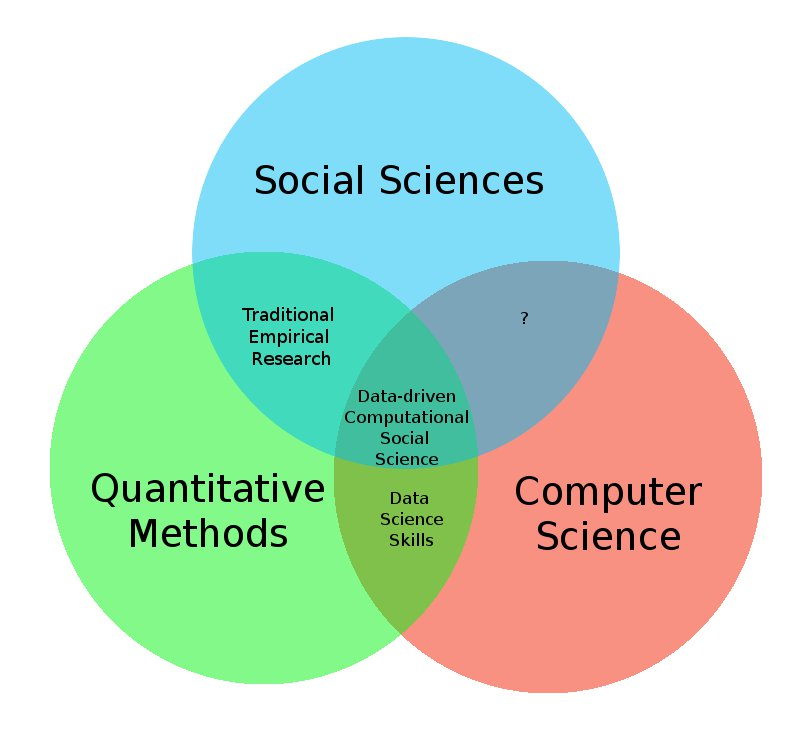
\includegraphics{../fig/ccsvenn.jpeg}

\end{frame}

\begin{frame}{Beispiele}

\begin{itemize}
\itemsep1pt\parskip0pt\parsep0pt
\item
  Demokratien führen keine Kriege gegeneinander.
\item
  Bürgerkriege finden eher in armen Ländern statt.
\item
  Negative Einstellungen gegenüber Flüchtlingen sind höher in Regionen
  mit hoher Arbeitslosigkeit.
\end{itemize}

\end{frame}

\begin{frame}{Beispiele - Daten}

\begin{enumerate}
\def\labelenumi{\arabic{enumi}.}
\itemsep1pt\parskip0pt\parsep0pt
\item
  Demokratien führen keine Kriege gegeneinander.
\end{enumerate}

\begin{itemize}
\itemsep1pt\parskip0pt\parsep0pt
\item
  Zwischenstaatliche Kriege in einem bestimmten Zeitraum, Dyaden der
  Kriegsparteien.
\item
  Politisches System der jeweiligen Staaten zu Kriegsbeginn (Kategorien:
  D/ND? Kontinuum?)
\item
  Möglicherweise noch Ursache/Anlass des Konflikts (eingeteilt in
  Kategorien?)
\end{itemize}

\end{frame}

\begin{frame}{Beispiele - Daten}

\begin{enumerate}
\def\labelenumi{\arabic{enumi}.}
\setcounter{enumi}{1}
\itemsep1pt\parskip0pt\parsep0pt
\item
  Bürgerkriege finden eher in armen Ländern statt.
\end{enumerate}

\begin{itemize}
\itemsep1pt\parskip0pt\parsep0pt
\item
  Alle Bürgerkriege als Universum der relevanten Fälle.
\item
  Armutsmaß je Land: z.B. BIP pro Kopf; Jahresdaten,
  Veränderungsraten\ldots{}
\end{itemize}

\end{frame}

\begin{frame}{Beispiele - Daten}

\begin{enumerate}
\def\labelenumi{\arabic{enumi}.}
\setcounter{enumi}{2}
\itemsep1pt\parskip0pt\parsep0pt
\item
  Negative Einstellungen gegenüber Flüchtlingen sind höher in Regionen
  mit hoher Arbeitslosigkeit.
\end{enumerate}

\begin{itemize}
\itemsep1pt\parskip0pt\parsep0pt
\item
  Repräsentative Meinungsdaten;
\item
  Arbeitslosenquoten;
\item
  möglichst disaggregiert auf Länder-/Kreis-/Gemeindeebene;
\item
  andere Einflüsse relevant? -\textgreater{} Kontrollvariablen
\end{itemize}

\end{frame}

\begin{frame}{Forschungsprozess}

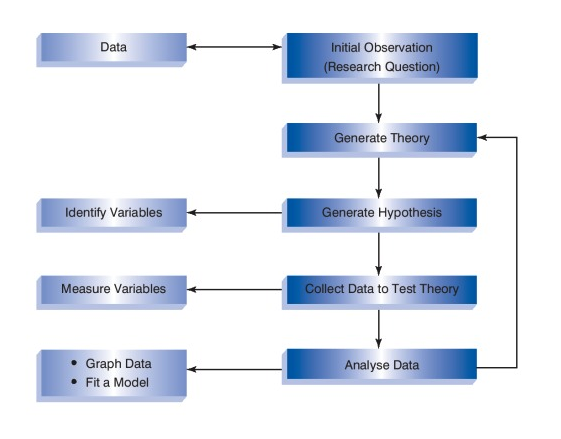
\includegraphics{../fig/research_process.png}

\tiny Quelle: Field, Miles, Field (2012): Discovering Statistics Using
R.

\end{frame}

\begin{frame}{Arbeitsprozess}

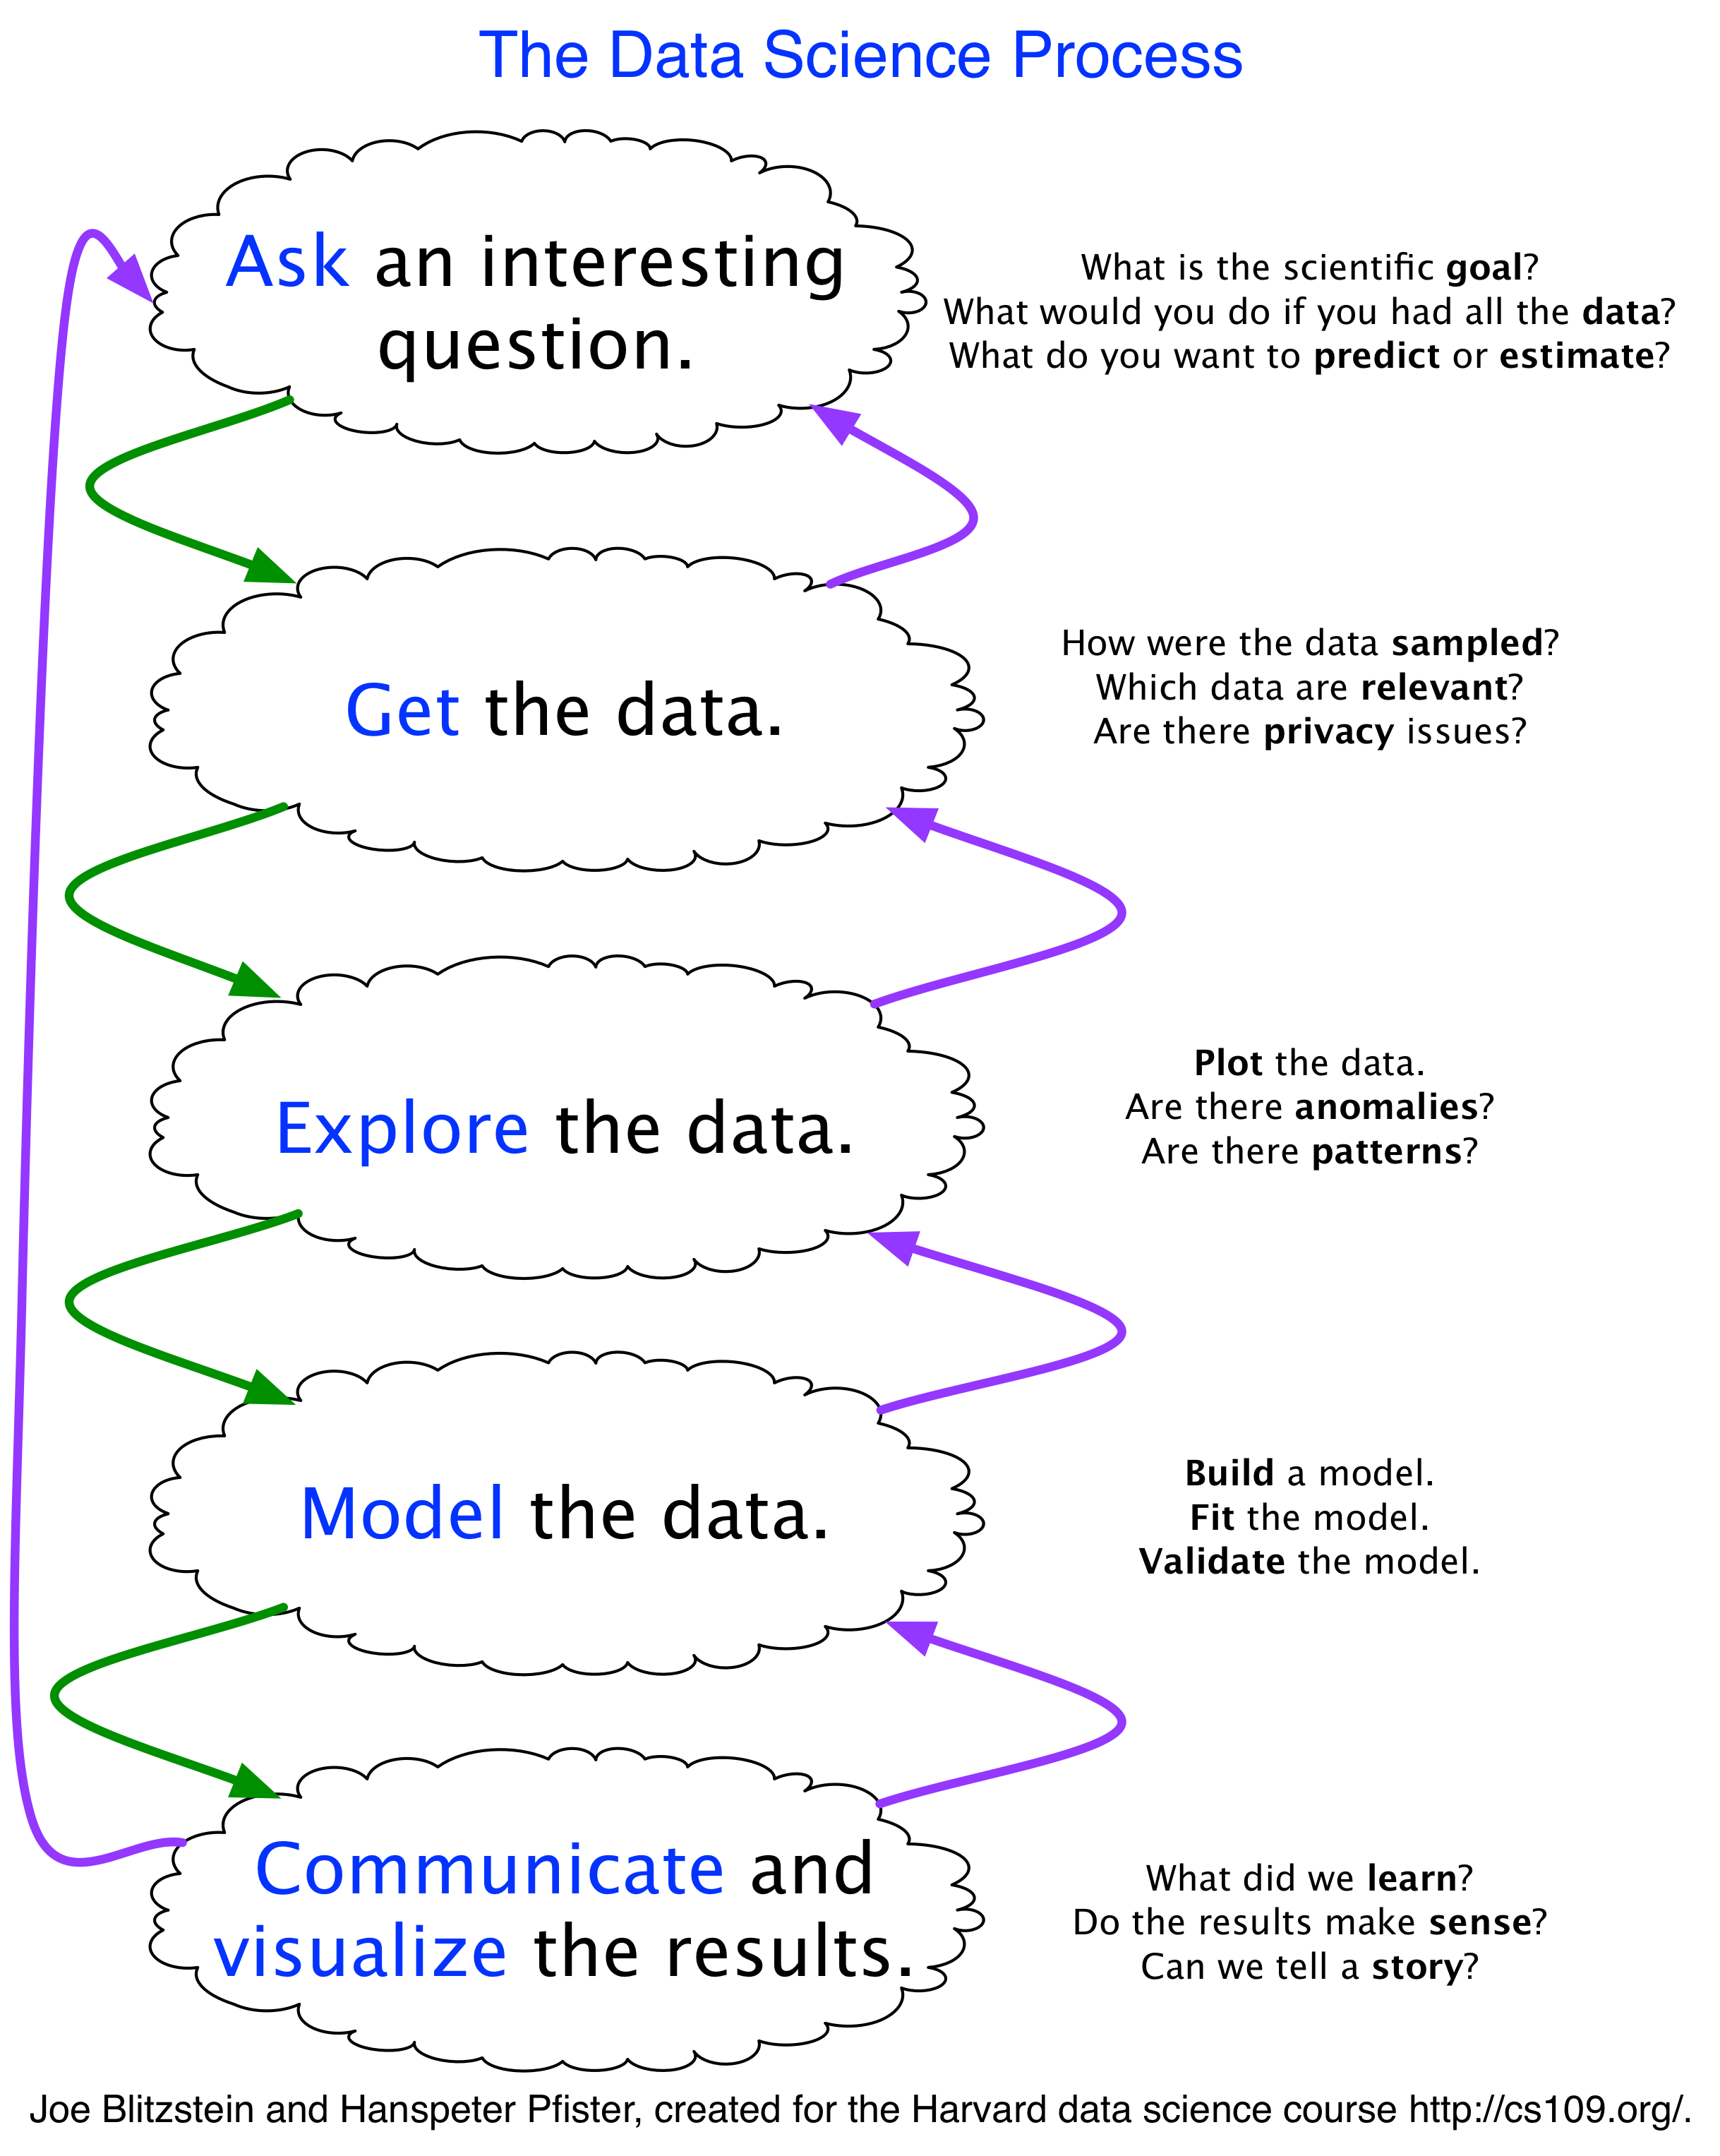
\includegraphics{../fig/data_science_workflow.png}

\end{frame}

\begin{frame}{Data Science}

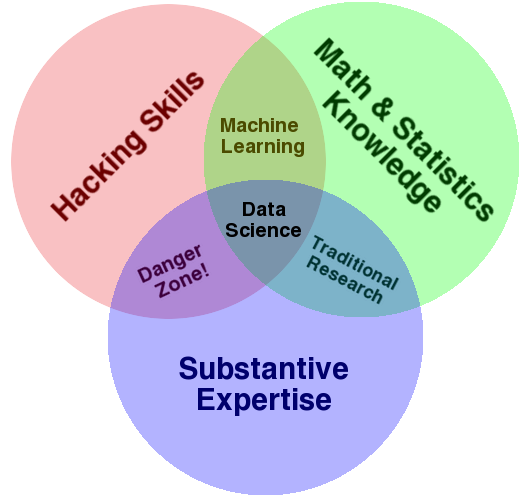
\includegraphics{../fig/data_science_VD.png}

\end{frame}

\begin{frame}{Weshalb benutzen wir spezielle Software?}

\begin{itemize}
\itemsep1pt\parskip0pt\parsep0pt
\item
  Excel reicht doch aus, um Daten zu verarbeiten, oder?
\item
  Nicht im wissenschaftlichen Sinne!
\item
  keine \textbf{Replizierbarkeit}
\item
  Umständliche Veränderungen vorheriger Schritte im
  Datenverarbeitungsprozess
\item
  komplexere Modelle, die über deskriptive Statistiken hinausgehen sind
  kaum möglich. Deshalb:
\item
  wissenschaftliche Statistiksoftware (z.B. Stata, Matlab, SPSS,
  EViews\ldots{})
\item
  wir nutzen in diesem Kurs R.
\end{itemize}

\end{frame}

\begin{frame}{Warum R?}

\begin{itemize}
\itemsep1pt\parskip0pt\parsep0pt
\item
  Freie Software.
\item
  Gewaltiger Funktionsumfang, der stetig erweitert und verbessert wird.
\item
  Zusätzliche Funktionen werden mithilfe von Paketen geladen. Diese sind
  über CRAN (Comprehensive R Archive Network) herunterzuladen.
\item
  Sehr aktive Community.
\item
  Hoher Verbreitungsgrad in Wissenschaft und wachsend in der Wirtschaft.
\end{itemize}

\end{frame}

\begin{frame}{R bei der NY-Times}

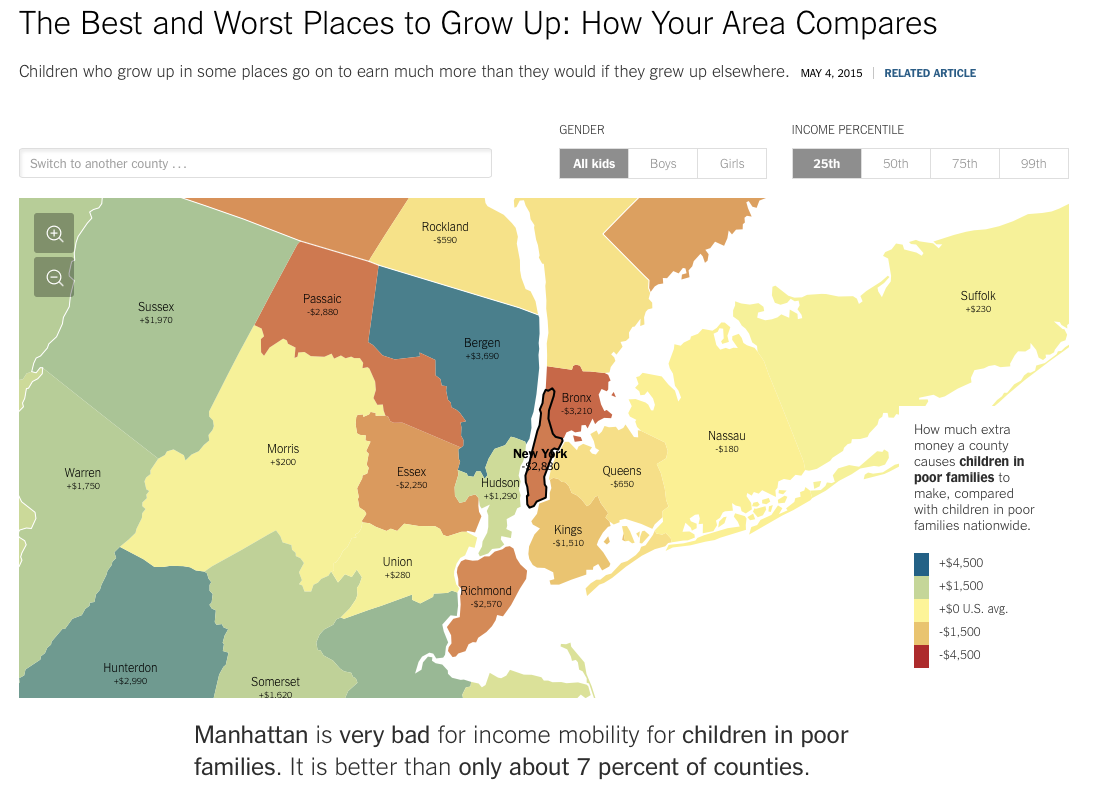
\includegraphics{../fig/ny-times.png}

\end{frame}

\begin{frame}{Persönlicher Nutzen}

\begin{itemize}
\itemsep1pt\parskip0pt\parsep0pt
\item
  R als universelles Werkzeug der Datenanalyse
\item
  Sie lernen durch die Programmiersprache strukturiert und analytisch zu
  denken.
\item
  R-Anwender sind gesucht!
\end{itemize}

\end{frame}

\begin{frame}{R auf dem Arbeitsmarkt}

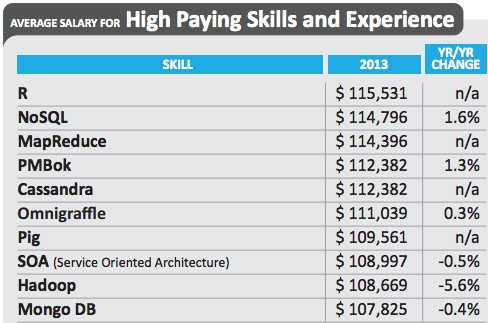
\includegraphics{../fig/skills_earnings.png}

\end{frame}

\begin{frame}{R auf dem Arbeitsmarkt}

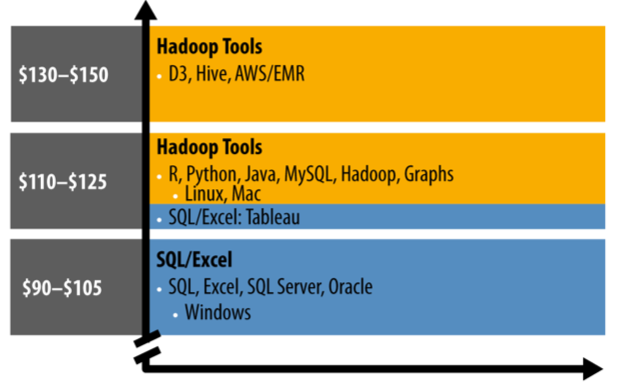
\includegraphics{../fig/skills_earnings_2.png}

\end{frame}

\begin{frame}{Hinweise für eine erfolgreiche Teilnahme}

\begin{itemize}
\itemsep1pt\parskip0pt\parsep0pt
\item
  Keine Pogrammierkenntnisse erforderlich (aber hilfreich).
\item
  Nachvollziehen und aktive Nutzung der Beispiele hilft Ihrem
  Lernprozess.
\item
  R ist eine Sprache:
\item
  Vokabeln
\item
  Grammatik
\item
  Fehler helfen beim Lernen!
\end{itemize}

\end{frame}

\begin{frame}{Organisatorisches}

Termine:

\begin{longtable}[c]{@{}rll@{}}
\toprule
\begin{minipage}[b]{0.18\columnwidth}\raggedleft\strut
Sitzung
\strut\end{minipage} &
\begin{minipage}[b]{0.18\columnwidth}\raggedright\strut
Datum
\strut\end{minipage} &
\begin{minipage}[b]{0.46\columnwidth}\raggedright\strut
Thema
\strut\end{minipage}\tabularnewline
\midrule
\endhead
\begin{minipage}[t]{0.18\columnwidth}\raggedleft\strut
1
\strut\end{minipage} &
\begin{minipage}[t]{0.18\columnwidth}\raggedright\strut
19.10.15
\strut\end{minipage} &
\begin{minipage}[t]{0.46\columnwidth}\raggedright\strut
Ziele quantitativer Forschung, Grundbegriffe der Datenanalyse
\strut\end{minipage}\tabularnewline
\begin{minipage}[t]{0.18\columnwidth}\raggedleft\strut
2
\strut\end{minipage} &
\begin{minipage}[t]{0.18\columnwidth}\raggedright\strut
26.10.15
\strut\end{minipage} &
\begin{minipage}[t]{0.46\columnwidth}\raggedright\strut
Einführung in R \& RStudio, grundlegende Funktionen
\strut\end{minipage}\tabularnewline
\begin{minipage}[t]{0.18\columnwidth}\raggedleft\strut
3
\strut\end{minipage} &
\begin{minipage}[t]{0.18\columnwidth}\raggedright\strut
02.11.15
\strut\end{minipage} &
\begin{minipage}[t]{0.46\columnwidth}\raggedright\strut
Statistische Grundlagen, Berechnung in R
\strut\end{minipage}\tabularnewline
\begin{minipage}[t]{0.18\columnwidth}\raggedleft\strut
4
\strut\end{minipage} &
\begin{minipage}[t]{0.18\columnwidth}\raggedright\strut
09.11.15
\strut\end{minipage} &
\begin{minipage}[t]{0.46\columnwidth}\raggedright\strut
Statistische Grundlagen, Berechnung in R
\strut\end{minipage}\tabularnewline
\begin{minipage}[t]{0.18\columnwidth}\raggedleft\strut
5
\strut\end{minipage} &
\begin{minipage}[t]{0.18\columnwidth}\raggedright\strut
16.11.15
\strut\end{minipage} &
\begin{minipage}[t]{0.46\columnwidth}\raggedright\strut
Deskriptive Statistiken und Datenvisualisierung
\strut\end{minipage}\tabularnewline
\begin{minipage}[t]{0.18\columnwidth}\raggedleft\strut
6
\strut\end{minipage} &
\begin{minipage}[t]{0.18\columnwidth}\raggedright\strut
23.11.15
\strut\end{minipage} &
\begin{minipage}[t]{0.46\columnwidth}\raggedright\strut
Plots und Datenverarbeitung
\strut\end{minipage}\tabularnewline
\begin{minipage}[t]{0.18\columnwidth}\raggedleft\strut
7
\strut\end{minipage} &
\begin{minipage}[t]{0.18\columnwidth}\raggedright\strut
30.11.15
\strut\end{minipage} &
\begin{minipage}[t]{0.46\columnwidth}\raggedright\strut
Datenverarbeitung
\strut\end{minipage}\tabularnewline
\bottomrule
\end{longtable}

\end{frame}

\begin{frame}{Organisatorisches II}

Termine:

\begin{longtable}[c]{@{}rll@{}}
\toprule
\begin{minipage}[b]{0.17\columnwidth}\raggedleft\strut
Sitzung
\strut\end{minipage} &
\begin{minipage}[b]{0.17\columnwidth}\raggedright\strut
Datum
\strut\end{minipage} &
\begin{minipage}[b]{0.58\columnwidth}\raggedright\strut
Thema
\strut\end{minipage}\tabularnewline
\midrule
\endhead
\begin{minipage}[t]{0.17\columnwidth}\raggedleft\strut
8
\strut\end{minipage} &
\begin{minipage}[t]{0.17\columnwidth}\raggedright\strut
07.12.15
\strut\end{minipage} &
\begin{minipage}[t]{0.58\columnwidth}\raggedright\strut
Lineare Regression
\strut\end{minipage}\tabularnewline
\begin{minipage}[t]{0.17\columnwidth}\raggedleft\strut
9
\strut\end{minipage} &
\begin{minipage}[t]{0.17\columnwidth}\raggedright\strut
11.01.16
\strut\end{minipage} &
\begin{minipage}[t]{0.58\columnwidth}\raggedright\strut
Logit-Modell
\strut\end{minipage}\tabularnewline
\begin{minipage}[t]{0.17\columnwidth}\raggedleft\strut
10
\strut\end{minipage} &
\begin{minipage}[t]{0.17\columnwidth}\raggedright\strut
18.01.16
\strut\end{minipage} &
\begin{minipage}[t]{0.58\columnwidth}\raggedright\strut
Zähl-Modell
\strut\end{minipage}\tabularnewline
\begin{minipage}[t]{0.17\columnwidth}\raggedleft\strut
11
\strut\end{minipage} &
\begin{minipage}[t]{0.17\columnwidth}\raggedright\strut
25.01.16
\strut\end{minipage} &
\begin{minipage}[t]{0.58\columnwidth}\raggedright\strut
Anwendungsbeispiele
\strut\end{minipage}\tabularnewline
\begin{minipage}[t]{0.17\columnwidth}\raggedleft\strut
12
\strut\end{minipage} &
\begin{minipage}[t]{0.17\columnwidth}\raggedright\strut
01.02.16
\strut\end{minipage} &
\begin{minipage}[t]{0.58\columnwidth}\raggedright\strut
Wiederholung/Fragestunde
\strut\end{minipage}\tabularnewline
\begin{minipage}[t]{0.17\columnwidth}\raggedleft\strut
13
\strut\end{minipage} &
\begin{minipage}[t]{0.17\columnwidth}\raggedright\strut
08.02.16
\strut\end{minipage} &
\begin{minipage}[t]{0.58\columnwidth}\raggedright\strut
Klausur: Replikation einer Studie
\strut\end{minipage}\tabularnewline
\bottomrule
\end{longtable}

\end{frame}

\begin{frame}{Organisatorisches III}

\begin{block}{Leistungsnachweis:}

\begin{itemize}
\itemsep1pt\parskip0pt\parsep0pt
\item
  Aufgabenblatt in der Weihnachtspause (25\%)
\item
  Klausur (auch eine Art Aufgabenblatt) (75\%)
\end{itemize}

\end{block}

\end{frame}

\begin{frame}{Organisatorisches IV}

\begin{itemize}
\item
  Folien über OLAT
\item
  Folien, Datensätze und Code auf Github:
  \href{http://www.github.com/davben/stats-with-r}{\url{http://www.github.com/davben/stats-with-r}}
\item
  Sprechstunde nach Vereinbarung:
  \href{mailto:david.bencek@ifw-kiel.de}{\nolinkurl{david.bencek@ifw-kiel.de}}
\end{itemize}

\end{frame}

\begin{frame}{Einstieg in R und RStudio}

\end{frame}

\end{document}